% xcolor and define colors -------------------------
\usepackage{xcolor}

% https://www.viget.com/articles/color-contrast/
\definecolor{purple}{HTML}{5601A4}
\definecolor{navy}{HTML}{0D3D56}
\definecolor{ruby}{HTML}{9a2515}
\definecolor{alice}{HTML}{107895}
\definecolor{daisy}{HTML}{EBC944}
\definecolor{coral}{HTML}{F26D21}
\definecolor{kelly}{HTML}{829356}
\definecolor{cranberry}{HTML}{E64173}
\definecolor{jet}{HTML}{131516}
\definecolor{asher}{HTML}{555F61}
\definecolor{slate}{HTML}{314F4F}

% Mixtape Sessions
\definecolor{picton-blue}{HTML}{00b7ff}
\definecolor{violet-red}{HTML}{ff3881}
\definecolor{sun}{HTML}{ffaf18}
\definecolor{electric-violet}{HTML}{871EFF}

\newcommand\pictonBlue[1]{{\color{picton-blue}#1}}
\newcommand\sun[1]{{\color{sun}#1}}
\newcommand\electricViolet[1]{{\color{electric-violet}#1}}
\newcommand\violetRed[1]{{\color{violet-red}#1}}

\newcommand\bgPictonBlue[1]{{\colorbox{picton-blue!20!white}{#1}}}
\newcommand\bgSun[1]{{\colorbox{sun!20!white}{#1}}}
\newcommand\bgElectricViolet[1]{{\colorbox{electric-violet!20!white}{#1}}}
\newcommand\bgVioletRed[1]{{\colorbox{violet-red!20!white}{#1}}}

\def\code#1{\texttt{#1}}

% Main theme colors
\definecolor{accent}{HTML}{00b7ff}
\definecolor{accent2}{HTML}{871EFF}
\definecolor{gray100}{HTML}{f3f4f6}
\definecolor{gray800}{HTML}{1F292D}


% Beamer Options -------------------------------------

% Background
\setbeamercolor{background canvas}{bg = white}

% Change text margins
\setbeamersize{text margin left = 15pt, text margin right = 15pt} 

% \alert
\setbeamercolor{alerted text}{fg = accent2}

% Frame title
\setbeamercolor{frametitle}{bg = white, fg = jet}
\setbeamercolor{framesubtitle}{bg = white, fg = accent}
\setbeamerfont{framesubtitle}{size = \small, shape = \itshape}

% Block
\setbeamercolor{block title}{fg = white, bg = accent2}
\setbeamercolor{block body}{fg = gray800, bg = gray100}

% Title page
\setbeamercolor{title}{fg = gray800}
\setbeamercolor{subtitle}{fg = accent}

%% Custom \maketitle and \titlepage
\setbeamertemplate{title page}
{
    %\begin{centering}
        \vspace{20mm}
        {\Large \usebeamerfont{title}\usebeamercolor[fg]{title}\inserttitle}\\
        {\large \itshape \usebeamerfont{subtitle}\usebeamercolor[fg]{subtitle}\insertsubtitle}\\ \vspace{10mm}
        {\insertauthor}\\
        {\color{asher}\small{\insertdate}}\\
    %\end{centering}
}

% Table of Contents
\setbeamercolor{section in toc}{fg = accent!70!jet}
\setbeamercolor{subsection in toc}{fg = jet}

% Button 
\setbeamercolor{button}{bg = accent}

% Remove navigation symbols
\setbeamertemplate{navigation symbols}{}

% Table and Figure captions
\setbeamercolor{caption}{fg=jet!70!white}
\setbeamercolor{caption name}{fg=jet}
\setbeamerfont{caption name}{shape = \itshape}

% Bullet points

%% Fix spacing between items
\let\olditemize=\itemize 
\let\endolditemize=\enditemize 
\renewenvironment{itemize}{\vspace{0.25em}\olditemize \itemsep0.25em}{\endolditemize}

%% Fix left-margins
\settowidth{\leftmargini}{\usebeamertemplate{itemize item}}
\addtolength{\leftmargini}{\labelsep}

%% enumerate item color
\setbeamercolor{enumerate item}{fg = accent}
\setbeamerfont{enumerate item}{size = \small}
\setbeamertemplate{enumerate item}{\insertenumlabel.}

%% itemize
\setbeamercolor{itemize item}{fg = accent!70!white}
\setbeamerfont{itemize item}{size = \small}
\setbeamertemplate{itemize item}[circle]

%% right arrow for subitems
\setbeamercolor{itemize subitem}{fg = accent!60!white}
\setbeamerfont{itemize subitem}{size = \small}
\setbeamertemplate{itemize subitem}{$\rightarrow$}

\setbeamertemplate{itemize subsubitem}[square]
\setbeamercolor{itemize subsubitem}{fg = jet}
\setbeamerfont{itemize subsubitem}{size = \small}








% Links ----------------------------------------------

\usepackage{hyperref}
\hypersetup{
  colorlinks = true,
  linkcolor = accent2,
  filecolor = accent2,
  urlcolor = accent2,
  citecolor = accent2,
}


% Line spacing --------------------------------------
\usepackage{setspace}
\setstretch{1.35}


% \begin{columns} -----------------------------------
\usepackage{multicol}


% Fonts ---------------------------------------------
% Beamer Option to use custom fonts
\usefonttheme{professionalfonts}

% \usepackage[utopia, smallerops, varg]{newtxmath}
% \usepackage{utopia}
\usepackage[sfdefault,light]{roboto}

% Small adjustments to text kerning
\usepackage{microtype}



% Remove annoying over-full box warnings -----------
\vfuzz2pt 
\hfuzz2pt


% Table of Contents with Sections
\setbeamerfont{myTOC}{series=\bfseries, size=\Large}
\AtBeginSection[]{
        \frame{
            \frametitle{Roadmap}
            \tableofcontents[current]   
        }
    }


% Tables -------------------------------------------
% Tables too big
% \begin{adjustbox}{width = 1.2\textwidth, center}
\usepackage{adjustbox}
\usepackage{array}
\usepackage{threeparttable, booktabs, adjustbox}
    
% Fix \input with tables
% \input fails when \\ is at end of external .tex file
\makeatletter
\let\input\@@input
\makeatother

% Tables too narrow
% \begin{tabularx}{\linewidth}{cols}
% col-types: X - center, L - left, R -right
% Relative scale: >{\hsize=.8\hsize}X/L/R
\usepackage{tabularx}
\newcolumntype{L}{>{\raggedright\arraybackslash}X}
\newcolumntype{R}{>{\raggedleft\arraybackslash}X}
\newcolumntype{C}{>{\centering\arraybackslash}X}

% Figures

% \imageframe{img_name} -----------------------------
% from https://github.com/mattjetwell/cousteau
\newcommand{\imageframe}[1]{%
    \begin{frame}[plain]
        \begin{tikzpicture}[remember picture, overlay]
            \node[at = (current page.center), xshift = 0cm] (cover) {%
                \includegraphics[keepaspectratio, width=\paperwidth, height=\paperheight]{#1}
            };
        \end{tikzpicture}
    \end{frame}%
}

% subfigures
\usepackage{subfigure}


% Highlight slide -----------------------------------
% \begin{transitionframe} Text \end{transitionframe}
% from paulgp's beamer tips
\newenvironment{transitionframe}{
    \setbeamercolor{background canvas}{bg=accent!40!black}
    \begin{frame}\color{accent!10!white}\LARGE\centering
}{
    \end{frame}
}


% Table Highlighting --------------------------------
% Create top-left and bottom-right markets in tabular cells with a unique matching id and these commands will outline those cells
\usepackage[beamer,customcolors]{hf-tikz}
\usetikzlibrary{calc}
\usetikzlibrary{fit,shapes.misc}

% To set the hypothesis highlighting boxes red.
\newcommand\marktopleft[1]{%
    \tikz[overlay,remember picture] 
        \node (marker-#1-a) at (0,1.5ex) {};%
}
\newcommand\markbottomright[1]{%
    \tikz[overlay,remember picture] 
        \node (marker-#1-b) at (0,0) {};%
    \tikz[accent!80!jet, ultra thick, overlay, remember picture, inner sep=4pt]
        \node[draw, rectangle, fit=(marker-#1-a.center) (marker-#1-b.center)] {};%
}


% DAGS ----------------------------------------------
\usepackage{tikz}
\usetikzlibrary{shapes,decorations,arrows,calc,arrows.meta,fit,positioning}
% Tikz settings optimized for causal graphs.
\tikzset{
    -Latex,auto,node distance =1 cm and 1 cm,semithick,
    state/.style ={ellipse, draw, minimum width = 0.7 cm},
    point/.style = {circle, draw, inner sep=0.04cm,fill,node contents={}},
    bidirected/.style={Latex-Latex,dashed},
    el/.style = {inner sep=2pt, align=left, sloped}
}


% Beamer tricks -------------------------------------
% Make \pause work in align environments
\makeatletter
\renewrobustcmd{\beamer@@pause}[1][]{%
  \unless\ifmeasuring@%
  \ifblank{#1}%
    {\stepcounter{beamerpauses}}%
    {\setcounter{beamerpauses}{#1}}%
  \onslide<\value{beamerpauses}->\relax%
  \fi%
}
\makeatother


\title [Nonparametrics]{Nonparametrics and Local Methods: Advanced Topics}
\author{C.Conlon}
\institute{Applied Econometrics}
\date{\today}
\setbeamerfont{equation}{size=\tiny}
\begin{document}

\begin{frame}
\titlepage
\end{frame}

\frame{\frametitle{Local Bandwidths}

\pause

If you only care about $f(y)$ at some given point, then 
\[
A=f''(y)^2 \left(\int u^2K\right)^2/4 \mbox{ and } B=f(y)\int K^2.
\]

\pause

So in a low-density region, worry about variance and take $h$ larger.
In a curvy region, worry about bias and take $h$ small.
 
}

\frame{\frametitle{Higher-Order Kernels}
\begin{itemize}
\item $K$ of order $r$ iff $\int x^j K(x) dx=0$ for $j<r$ and $\int x^r
K(x)dx \neq 0$. Try $r>2$?
\item The beauty of it: bias in $h^r$ if $f$ is at least $C^r$\ldots so AMISE can be
reduced to $n^{-r/(2r+1)}$, almost $\sqrt{n}$-consistent if $r$ is
large. 
\item But gives wiggly (and sometimes negative) estimates
$\rightarrow$ leave them to theorists. 
\end{itemize}
}

\begin{frame}{Back to the CDF}
\small
Since now we have estimated the density with
\begin{align*}
{\hat f}_n(y)= \frac{1}{nh}\sum_{i=1}^n K\left(
\frac{y-y_i}{h}\right),
\end{align*}
a natural idea is to integrate; let $\mathcal{K}(y)=\int_{-\infty}^y K(t)dt$, try
\begin{align*}
{\hat F}_n(y)= \frac{1}{n}\sum_{i=1}^n \mathcal{K}\left(
\frac{y-y_i}{h}\right)
\end{align*}
as a reasonable estimator of the cdf in $y$.
Very reasonable indeed:
\begin{itemize}
  \item when $n \longrightarrow \infty$ and $h$ goes to zero (at rate
    $n^{-1/3}$\ldots) 
it is consistent at rate $\sqrt{n}$
\item it is nicely smooth and accords well with the density estimator
\item \ldots\ it is a much better choice than the empirical cdf.
\end{itemize}
\end{frame}


\frame{\frametitle{What if $y$ is of dimension $p_y>1$?}

\pause

``Easy'': use $p_y$-dimensional $K$ (often a $p_y$-product of 1-dim
kernels) and bandwidth $h$, and do

\pause


\[
{\hat f}_n(y)= \frac{1}{nh^p_y}\sum_{i=1}^n K\left(
\frac{y-y_i}{h}\right).
\]

\begin{itemize}
\item {\bf 1st minor pitfall:} the various dimensions may have very
different variances, so use  $(h_1,\ldots,h_{p_y})$.
\item {\bf 2nd minor pitfall:} they may be strongly correlated; then
sphericize first.
\item {\bf Major problem:} next slide\ldots
\end{itemize}
 }

 \frame{\frametitle{The Curse of Dimensionality}

\pause

\begin{itemize}
\item Computational cost increases exponentially.
\item {\em Much worse:} to achieve precision $\epsilon$ in dimension $p_y$, the number of
  observations you need increases as
\[
n \simeq \epsilon^{-(2+p_y/2)}.
\]
\item The {\em empty space\/} phenomenon: 
if $(y_1,\ldots,y_{p_y})$ all are iid uniform on $[-1,1]$, then only
$n/(10^{p_y})$ observations on average have all components in
$[-0.1,0.1]$. Bias still in $h^2$, but variance in $1/nh^{p_y}$ now.
\end{itemize}
}

\frame{\frametitle{Silverman's Table}

\pause

 Silverman (1986 book) 
provides a table illustrating the difficulty of kernel estimation
in high dimensions. To estimate the density at 0 of a $N(0,1)$ with
a given accuracy, he reports:

\pause

\begin{table}
\begin{center}
\vspace{1ex}
\begin{tabular}{|c|c|}\hline
Dimensionality Required & Sample Size    \\
\hline
1               &  4    \\
2               &  19    \\
5           & 786 \\
7          & 10,700 \\
10           & 842,000 \\
\hline
\end{tabular}
\end{center}
\end{table}

\pause

{\bf Not to be taken lightly\ldots} in any case convergence  with
the optimal bandwidth  is in $n^{-2/(4+p_y)}$ now---and Silverman's
rule of thumb for choosing $h^*_n$ must be adapted too. }

\frame{\frametitle{Usually we care about conditional densities}

\pause

That is: we have covariates $x$, we want the density $f(y|x)$. Again, ``easy'':

\pause

\begin{enumerate}
\item get a kernel estimator of the joint density $f(y,x)$;
\item and one of of the marginal density $f(x)$;
\item then define
\[
\hat{f}_n(y|x)=\frac{\hat{f}_n(y,x)}{\hat{f}_n(x)}=\frac{\frac{1}{n
h_y^{p_y}h_x^{p_x}}\sum_{i=1}^n
K\left(\frac{y-y_i}{h_y}\right)K\left(\frac{x-x_i}{h_x}\right)}{\frac{1}{h_y^{p_y}}
\sum_{i=1}^n K\left(\frac{x-x_i}{h_x}\right)}.
\]
\end{enumerate}

\pause

But the joint density is $(p_x+p_y)$ dimensional\ldots\ and the curse
strikes big time.

}





\frame{\frametitle{Nonparametric Regression}

\pause

Data $(y_i,x_i)_{i=1}^n$ now, we are after $E(g(y,x)|x)=m(x)$ for
some function $g$.
\begin{itemize}
\item Best-fit approach, quite unbiased:
\begin{itemize}[<+->]
\item
if $x=x_i$ then ${\hat m}_n(x)=g(y_i,x_i)$; otherwise \ldots whatever.
\end{itemize}
 But: very jagged estimate; variance independent of $n$, so not
consistent.
\item Better and most usual: Nadaraya-Watson, inspired from kernel idea:
\[
{\hat m}_n(x)=\frac{\sum_{i=1}^n g(y_i,x_i)
K\left(\frac{x-x_i}{h}\right)}{\sum_{i=1}^n
K\left(\frac{x-x_i}{h}\right)}.
\]
again, bias in $h^2$ and variance in $1/nh$ if $p_x=1$.

\pause

{\em Pitfall 1:} very unreliable where  $f(x)$ is small.

\pause

{\em Pitfall 2:} the formal for the optimal bandwidth $h$  is very ugly.
\end{itemize}
}

\frame{\frametitle{Choosing $h$}
\begin{itemize}
\item Plug-in estimates work badly.
\item Fortunately, cross-validation amounts to
\[
\min_h \sum_{i=1}^n
\frac{\left(g(y_i,x_i)-\hat{m}_n(x_i;h)\right)^2}{1-k_i(h)}
\]
where $k_i(h)=K_h(0)/\sum_{j=1}^n K_h(x_i-x_j).$ 
\item So not that hard, and can be done on a subsample and rescaled.
\end{itemize}
}

\frame{\frametitle{Local Linear Regression}
\begin{itemize}
\item The Nadaraya-Watson  estimator in $x$ can be obtained very simply by regressing $g(y_i,x_i)$ on 1, weighting each
observation by $K((x-x_i)/h)$.
\item We could also regress on 1 and  $(x-x_i)$ (going to  higher terms
has problems) instead;\\
Advantages:
\begin{itemize}
\item the bias becomes 0 if the true $m(x)$ is linear.
\item the coefficient of $(x-x_i)$ estimates $m'(x)$.
\item behaves better in ``almost empty'' regions.
\end{itemize}
{Disadvantages:} hardly any, just do it!
\end{itemize}

 }
 
 \begin{frame}{Local Linear}
\begin{figure}[htbp]
\begin{center}
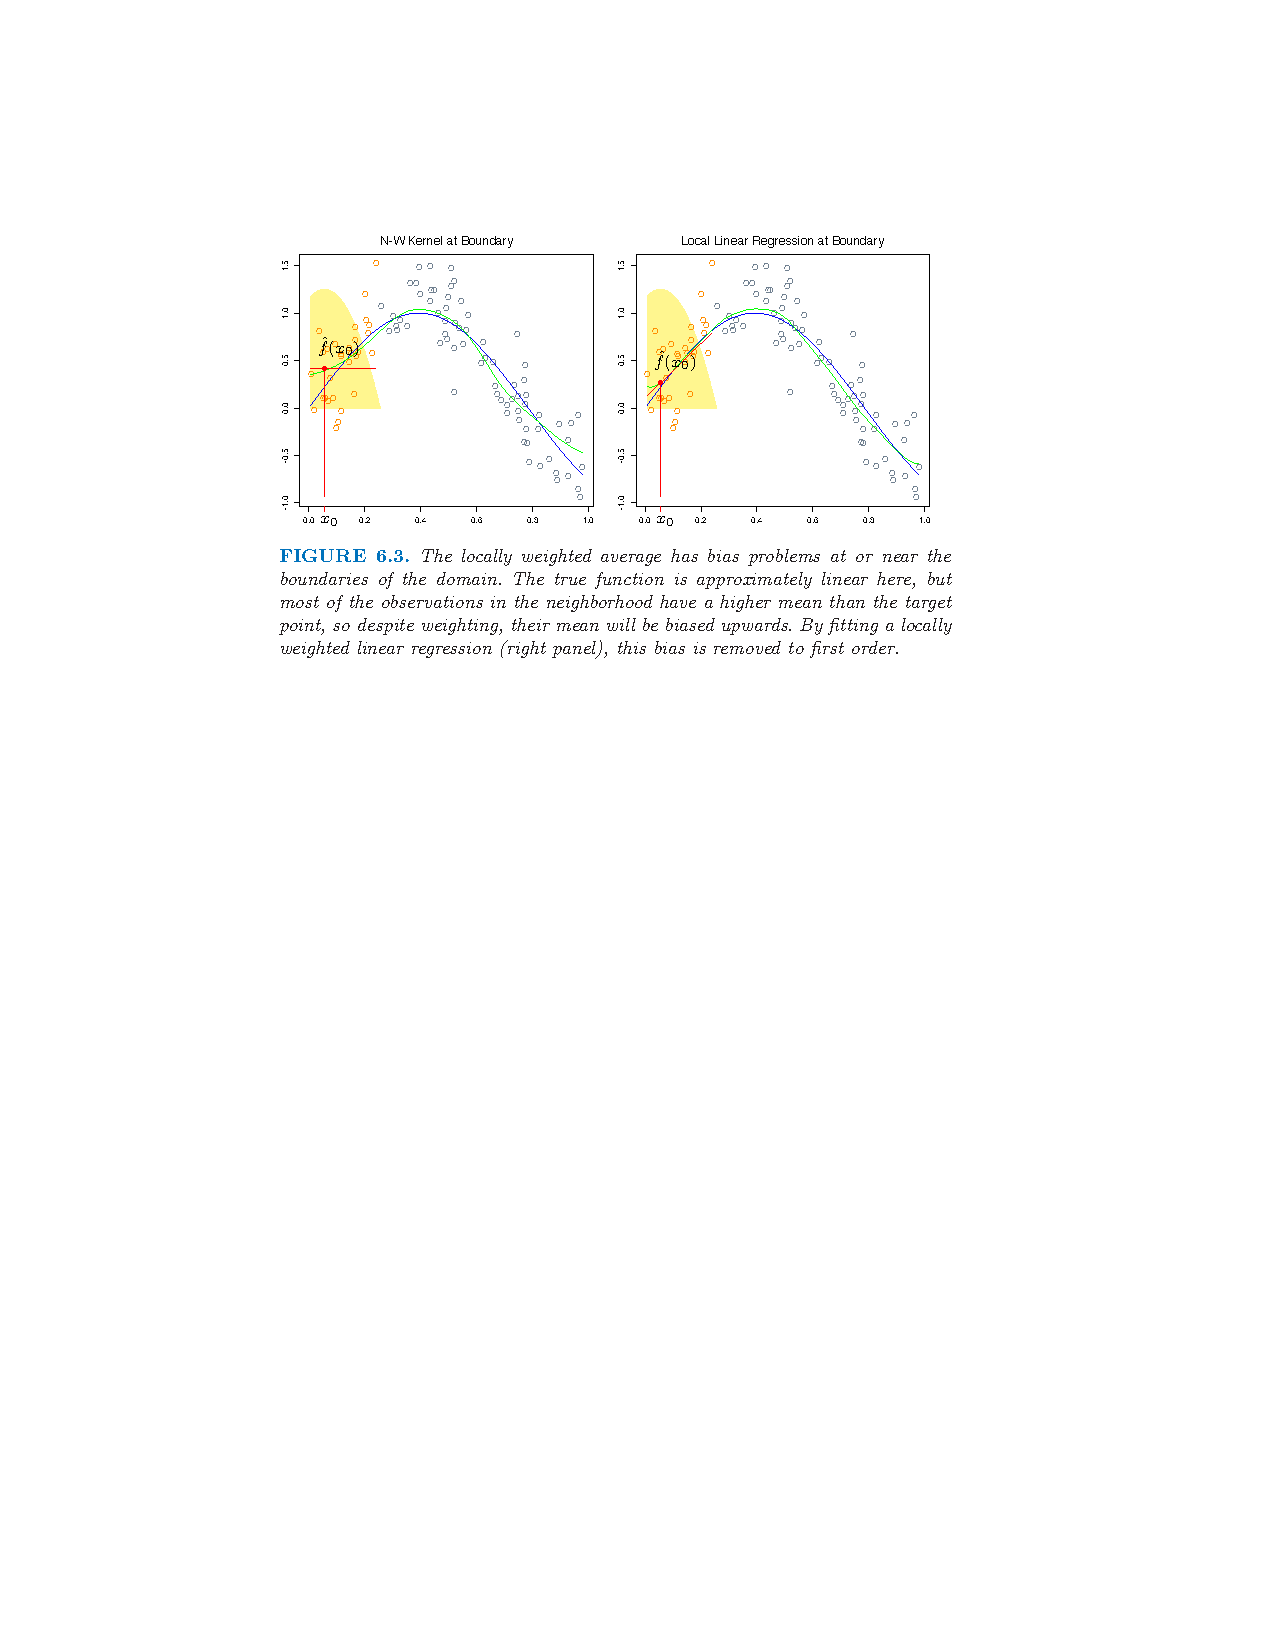
\includegraphics[width=3.5in]{./resources/nwloclinear.pdf}
\label{loclinear1}
\end{center}
\end{figure}
\end{frame}

 \begin{frame}{Local Linear}
\begin{figure}[htbp]
\begin{center}
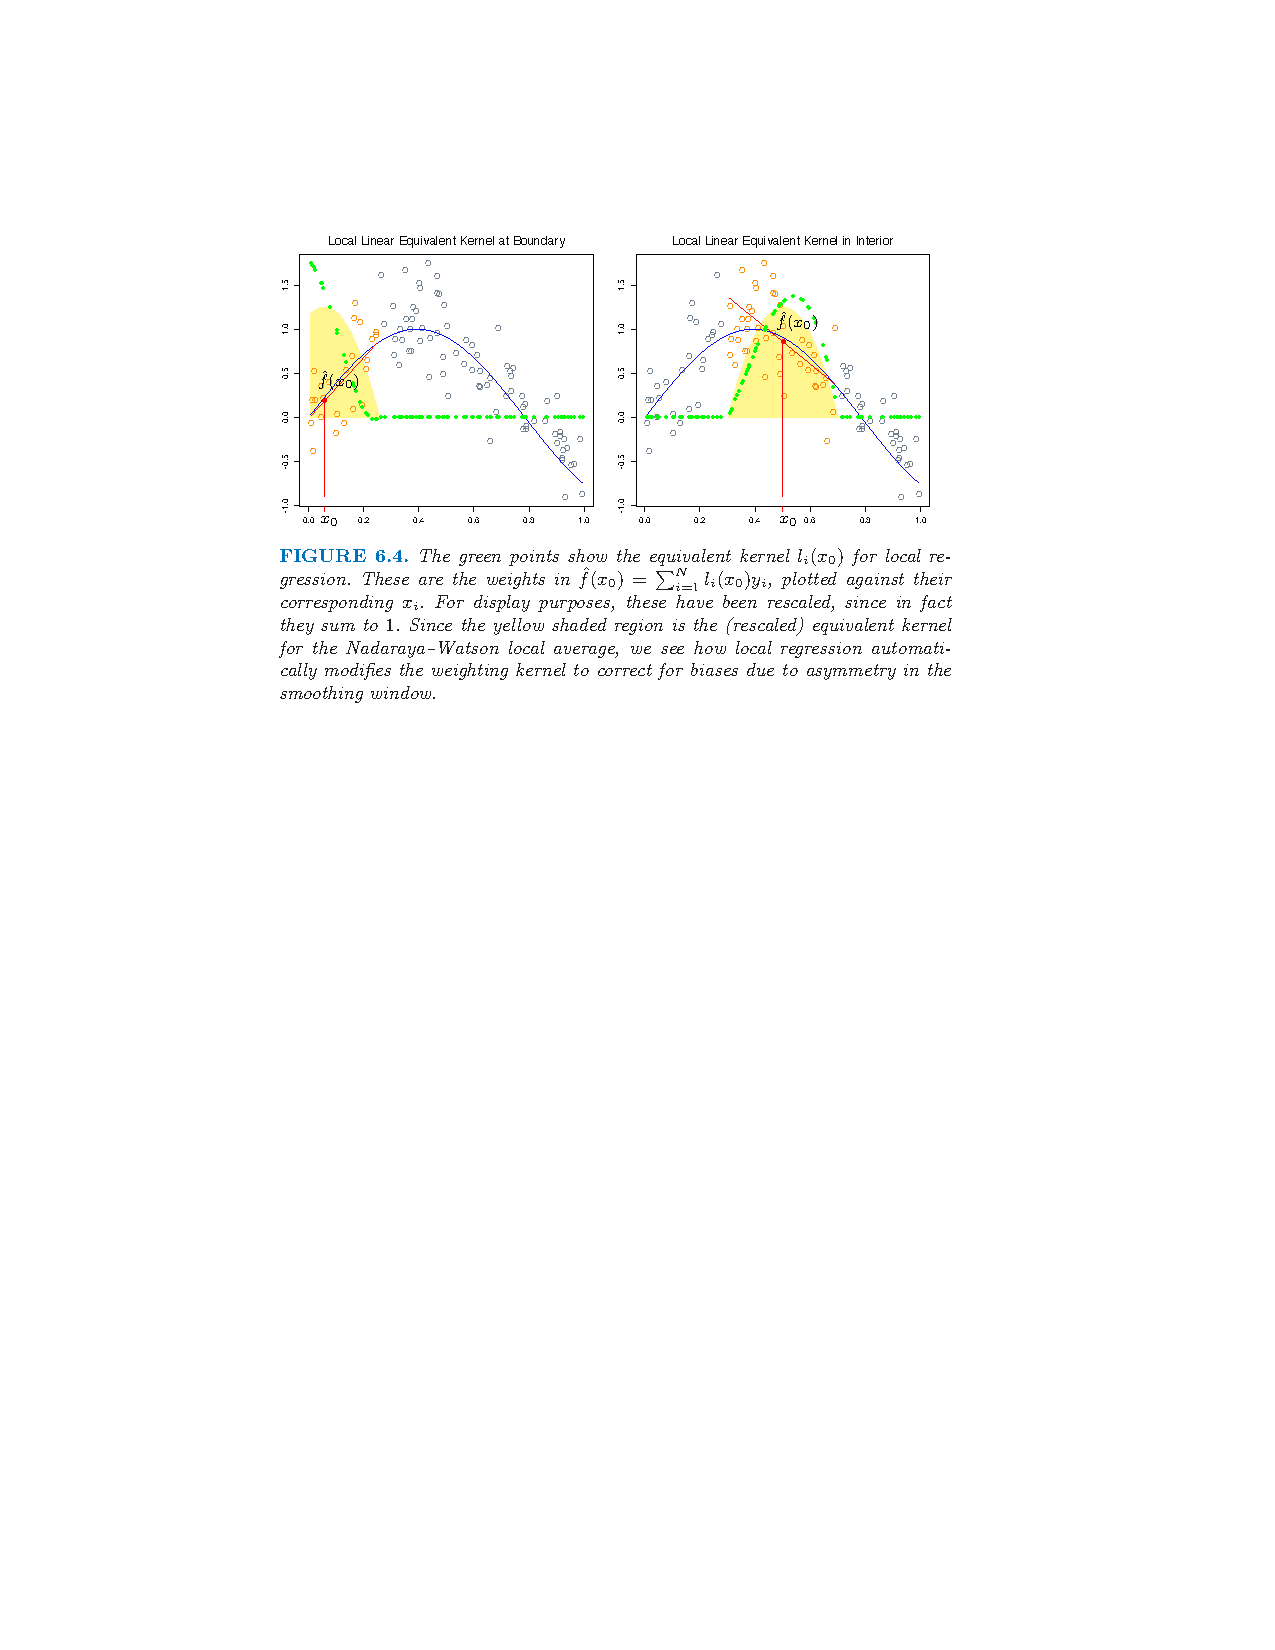
\includegraphics[width=3.5in]{./resources/nwloclinear2.pdf}
\label{loclinear2}
\end{center}
\end{figure}
\end{frame}


\begin{frame}{Local Quadratic}
\begin{figure}[htbp]
\begin{center}
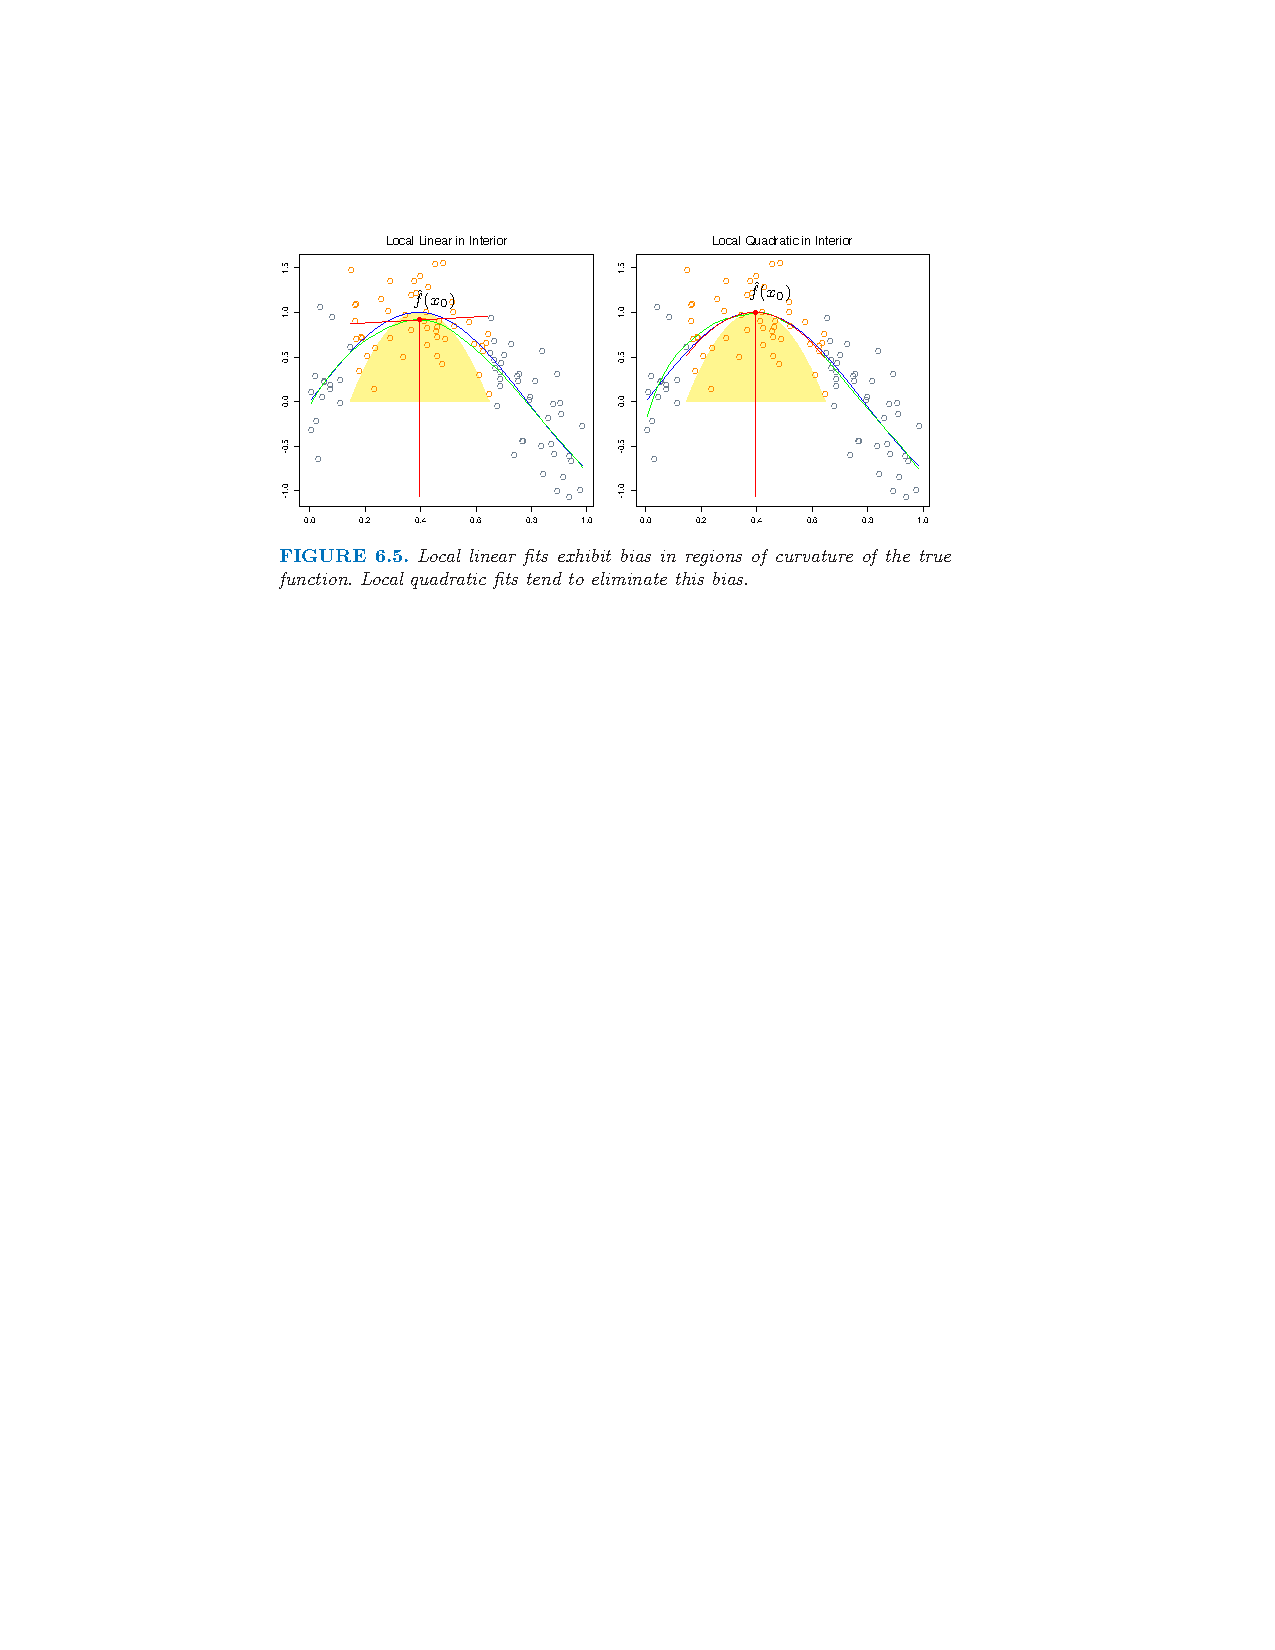
\includegraphics[width=3.5in]{./resources/locquad.pdf}
\label{loclinear2}
\end{center}
\end{figure}
\end{frame}

\frame{\frametitle{Nonparametric Regression, summary, 1}
Nadaraya--Watson for $E(y\vert x)=m(x)$ 
\[
\hat{m}(x)=\frac{\sum_i y_iK_h(x-x_i)}{\sum_i K_h(x-x_i)}
\]
\begin{itemize}
\item bias in $O(h^2)$, variance in $1/(nh^{p_x})$  
\item optimal $h$ in
$n^{-1/(p+4)}$: then bias, standard error and RMSE all converge at
rate $n^{-2/(p+4)}$
\item to select $h$, no rule of thumb: cross-validate on a subsample and
scale up.
\end{itemize}
}

\frame{\frametitle{Nonparametric Regression, summary, 2}
Nadaraya--Watson=\textbf{local constant regression}:  to get $\hat{m}(x)$,

\begin{enumerate}[<+->]
  \item  regress $y_i$ on $1$ with weight $K_h(x-x_i)$
\item take the estimated coeff as your $\hat{m}(x)$.
\end{enumerate}
Better: \textbf{local linear regression}
\begin{enumerate}[<+->]
  \item  regress $y_i$ on $1$ and $(x_i-x)$ with weight $K_h(x-x_i)$
\item take the estimated coeffs as your $\hat{m}(x)$ and $\hat{m}^\prime(x)$.
\end{enumerate}

To estimate the standard errors: bootstrap on an \emph{undersmoothed}
estimate (so that bias is negligible.)
}





\frame{\frametitle{What if my distribution is discrete-continuous?}
Very often in microeconometrics some covariates only take discrete
values (e.g. gender, race, income bracket\ldots). Say the only discrete variable is gender, we care about the density of income of men. 
\begin{itemize}
\item The kernel approach adapts directly: we separately
estimate a density for men (on the corresponding subsample).
\item {\em Better:}  mix the two subsamples! Add women, but  {\bf with a small weight $w$}.
\item Intuition: by doing so we increase the bias (the density for women is
probably different than for men) $\rightarrow$  bad, in $w^2$ but we reduce the variance, by $O(w)$; and this dominates for small $w$. (cf Li-Racine).
\end{itemize}
}
\begin{frame}{Review: What was the point?}
\begin{itemize}
\item OLS is lowest variance among linear unbiased estimators.
\item But there are \alert{nonlinear} estimators and potentially \alert{biased} estimators.
\begin{itemize}
\item Everything faces a \alert{bias-variance} tradeoff.
\item Nearly anything can be written as Kernel.
\end{itemize}
\end{itemize}

\end{frame}



\end{document}


